%!TEX root = ../thesis.tex
\chapter{Introduction}
\label{chapter:introduction}

% Personal fabrication machines, such as 3D printers, allow users to make custom objects. While early work on 3D printing revolved around designing the outside of such objects [24, 32], recently researchers started exploring 3D printing as a means to design the \textit{inside} of objects. Applications include moving objects’ centers of gravity so as to make them stand [20] or spin [1].


% The recent rise of widely accessible fabrication machines, such as 3D printers or laser cutters, generated interest in non-experts to create and design their own devices. Their strive towards a future of personal- rather than mass-fabrication is supported by HCI researchers [4], who investigate techniques to directly interact with the machine [29][32][50], use real-world objects for content creation [48][49] or embed mechanisms [52] and electronics [38]. These works were mainly concerned with creating the outside shape of 3D objects.

% 3D printing technology, however, is unique in that it allows users to freely arrange matter in space. Researchers used this property to generate internal structures that, e.g., optimize the strength-to-weight ratio of 3D objects [25], allow arbitrarily shaped objects to spin [3], or to float in pre-defined poses [34].

% Pushing this idea further, researchers engineer microstructures that deform in a desired way. These structures are usually arranged on a regular grid and together define the properties of the material they form [5]. This concept is known as metamaterials. Such metamaterial structures can be designed to change the materials’ elasticity [40], to absorb energy [12][43], or to change their shape [28]. 

% Recently, Ion et al. [18] pushed the concept of metamaterials further by going beyond materials and create complete mechanisms from cellular structures. Their mechanisms consist of two types of cells that are carefully arranged to move in concert to achieve the macroscopic mechanical movement. With their novel concept, they showed example objects including a door latch or a Jansen walker. However, it remains unclear what types of mechanisms can be implemented with such metamaterials.


Personal fabrication machines, such as 3D printers, have increasing impact on many areas including academia, aerospace industry, clothing or simply end-user products. The reason why 3D printing is so influential is that, in contrast to other manufacturing technologies such as CNC milling, molding, forming or laser cutting, 3D printing is the only technology that allows us to \textit{arrange matter freely in space.} A 3D printer is a generic machine that creates a physical representation of potentially any digital 3D model that users design. Such machines usually start with an empty build space and build up the object layer by layer. Due to this layer-by-layer approach the tool head that extrudes material always has access to the object and can dispose material anywhere on top of the last layer, which allows for arbitrary complexity. 

Naturally, the first 3D prints revolved around arbitrary shapes. However, researchers quickly found that by leveraging the freedom in material arrangement and altering how the material on the inside of objects is distributed, unique physical properties in their printed artifacts are enabled.



% This recent rise of widely accessible fabrication machines, sparked interest in non-expert users to create and design their own 3D objects and devices. 3D printing is unique in that it allows us to \textit{arrange matter freely in space.} Such machines usually start with an empty build space and build up the object layer by layer. Due to this layer-by-layer approach the tool head that extrudes material always has access to the object and can dispose material anywhere on top of the last layer, which allows for arbitrary complexity. Subtractive fabrication processes, such as milling, do not allow for such complexity. They start with a block of material and carve areas away, which means that the tool head must have access to those areas. This is the limiting factor of subtractive fabrication.

% In its current state, 3D printing is not free of limitations. While printing speed and support structures for overhangs are limitations of the technology itself, the design process for 3D objects that should be printed also still presents a big challenge. Generic computer-aided design (CAD) tools are powerful and complex expert tools and hard to learn for novice users. And the low speed of the fabrication process makes discovering errors slow, as users need to wait for many hours to test their design. Fortunately, due to the freedom that 3D printing brings in creating complex physical objects, researchers are determined to overcome these challenges and push 3D printing further by building systems that make this technology more accessible to experts as well as novice users.

% are very interested in optimizing the processes of content creation, in condensing the iteration cycles and in allowing users to create complex structures that improve their objects. 

% One limitation is that is usually slow, e.g., a printing a $10 \times 10\, \mathrm{mm}$ piece can take about 20 hours. Furthermore, overhanging structures must be supported with material that is to be removed later. This is mostly done by solid structures that are broken away mechanically, structures that are dissolved chemically, or powder that is blown out. The removal of support structures adds to the overall fabrication time. Another challenge in the current state of 3D printing is also the design process. The software tools for 3D modelling are often hard to master for inexperienced users. Fortunately, due to the freedom that 3D printing brings in creating complex physical objects, researchers investigate systems to overcome these challenges and push 3D printing further.

% Since 3D printing offers more freedom in creating complex physical objects, it helped researchers push the boundaries of technology by enabling them prototype their ideas directly. At the same time, 3D printers became cheaper and widely accessible to early adopters or so-called makers. 


\subsubsection{From the outside shape...}

Researchers in human-computer interaction started early on to investigate fabrication systems that are accessible for novice users. They reduced the hurdle of designing 3D models by presenting sketch-based CAD tools. Furthermore, researchers also enabled interactive fabrication systems by allowing users to directly interact with the machine \cite{Willis2011a, Mueller2012a, Peng2016}, increasing the number of iteration cycles \cite{Mueller2014, Mueller2014a}, use real-world objects for content creation \cite{Weichel2014, Weichel2015}, embed mechanisms \cite{Zhang2017} and electronics \cite{Weichel2013, Ledo2017}, or even fabricate things on the go \cite{Roumen2016}. These were mainly concerned with creating the outside shape of 3D models.


\subsubsection{to internal material distribution...}

Since 3D printing allows for creating physical objects with complex geometry, researchers investigated the redistribution of material on the inside of objects. They proposed tools to save material by optimizing the strength to weight ratio of 3D objects \cite{Lu2014}, allow arbitrarily shaped objects to spin reliably \cite{Bacher2014a}, or to float in pre-defined poses \cite{Prevost2016}. The availability of commercial tools \cite{AutodeskNetfabb2018, AutodeskWithin2018} to calculate the optimal material distribution for static objects even let industry adopt 3D printing as a production technique for special parts \cite{Sclupteo2018}.


\subsubsection{...to engineered microstructures}

Researchers in physics and mechanical engineering work on a similar concept, but they push the boundaries of engineered structures even further. They started to divide materials into a large number of cells on a regular grid. Since each cell is designed to perform a specific deformation \cite{Overvelde2012a}, objects that entirely consist of such cells literally offer thousands of degrees of freedom. Such structures are also known as mechanical \textit{metamaterials.} Metamaterials are artificial structures with mechanical properties that are defined by their usually repetitive cell patterns, rather than the material they are made of \cite{Bertoldi2017, Christensen2015, Paulose2015}.

Such metamaterials can exhibit extreme properties. Researchers developed nano-structures that yield ultra-lightweight materials \cite{Meza2014, Meza2015}, they investigated structures that can change their volume, i.e., they expand in two dimensions upon one-dimensional extension (so-called `auxetics' \cite{Lakes1987, Bertoldi2010, Jiang2018}), recoverable materials that damp impacts \cite{Frenzel2016a, Shan2015}, and even materials that hide enclosed objects from being felt \cite{Buckmann2015a}, that are tunable wave guides \cite{Babaee2016, Memoli2017} or as a thermal conductance managing materials \cite{Phoenix2017}. As these examples demonstrate, metamaterials allow researchers to create materials with very desirable and controllable
%\footnote{also referred to as `programmable'} 
properties.

% \begingroup
% \leftskip=2em
% % \rightskip=\leftskip
% \textbf{So far, metamaterials have been understood as materials. The main contribution of this thesis is that we think of them as \textit{devices.}}
% \par
% \endgroup

\singlespacing
\begin{siderule}
\large\textbf{So far, metamaterials have been understood as \mbox{materials.} The main contribution of this thesis is that we think of them as \textit{devices.}}
\end{siderule}
\onehalfspacing

% \pagebreak


\section{Metamaterial devices}

While metamaterials were already demonstrated to create materials with extreme properties, we push the field further by creating metamaterials that function like devices. The functionality of our metamaterial devices is solely defined by their cell geometry. We build devices from cells that \textit{play together} in a well-defined way to create interactive devices without electronics, but are purely defined by their material structure. The key benefit of our approach is that the resulting devices can be 3D printed from a single material and in one piece and thus do not require assembly. This means that they can be 3D printed as a part of a larger structure, such as full door including handle, latch mechanism and lock.

% We thereby blur the lines between materials and machines.

To instantiate this concept of metamaterial devices, we took inspiration from the input-process-output model. In this thesis, we present novel cell structures that implement mechanical devices that can process and output information depending on mechanical input from the user. 

\begin{figure} [h] %[h!|H] 
    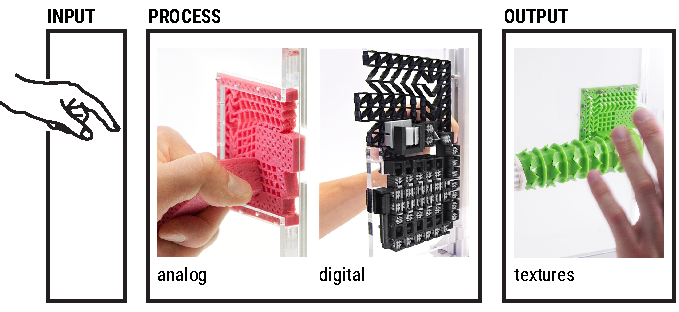
\includegraphics[width=\textwidth]{chapters/introduction-FIG/1-input-process-output.pdf}
    \caption[Short figure name.]{Metamaterial devices can process users' input and output to them again, thereby implementing an \textit{input-process-output} system without electronics, but purely within the material structure.
    \label{fig:1-overview-input-process-output-model}}
\end{figure}

Figure \ref{fig:1-overview-input-process-output-model} illustrates the core areas that we investigated in this thesis: we show (1) how we process \textit{analog} information in the context of metamaterials that transform forces and movements input by the user into a different set of forces and movement (i.e., mechanisms, (2) a system of cells that process information \textit{digitally}, and (3) cells that output information to the user or interface with the environment by appropriating dynamic textures.

Since designing such complex systems of cell structures is difficult, we additionally focus our work on providing accessible software to enable users to create such metamaterial devices.

% \begin{enumerate}
%     \item We integrate mechanisms within the material structure. Such metamaterial mechanisms consist of a single block of material the cells of which play together in a well-defined way in order to achieve macroscopic movement. This allows us to implement, e.g. a door latch, pliers, or a drawing machine from only one piece, without moving parts. 
    
%     \item Going beyond mechanical functions, we explore how to embody mechanical computation into 3D printed objects, i.e., without electronic sensors, actuators, or controllers typically used for this purpose. We demonstrate interactive objects based on this concept, such as a combination lock that are printed in one piece.
    
%     \item To further enhance 3D printed objects, we use metamaterials to change their outside. Such metamaterial textures can perform a controlled transition between two or more textures to allow designers to shape how objects interact with the environment and with the tactile sense of the user. 
% \end{enumerate}

% since we want to create interactive objects, we generally let the user provide input to our systems. 



\subsection{Processing analog signals}
We push the concept of metamaterials further by creating metamaterials that implement devices that transform input forces and movement into a desired set of output forces and movement---also known as mechanisms. Such metamaterial mechanisms consist of a single block of material the cells of which play together in a well-defined way in order to achieve macroscopic movement.

Figure \ref{fig:2-overview-metamaterial-mechanisms} shows an example of a metamaterial mechanism: a door latch mechanism. Our metamaterial door latch transforms the rotary movement of its handle into a linear motion of the latch. The key to transforming analog input are our shearing cells as they are only able to shear when subjected to an external force and thereby apply a controlled force to their neighboring cells.  While the traditional door latch mechanism consists of several parts, including an axle, bearings, springs, etc., the metamaterial door latch in Figure \ref{fig:2-overview-metamaterial-mechanisms} consists of a single block of material, as it is groups of cells inside the object that perform the mechanical function.
% The key element behind our metamaterial mechanisms is a specialized type of cell, the only ability of which is to shear. 

\begin{figure} [h] %[h!|H]
    \centering
    % 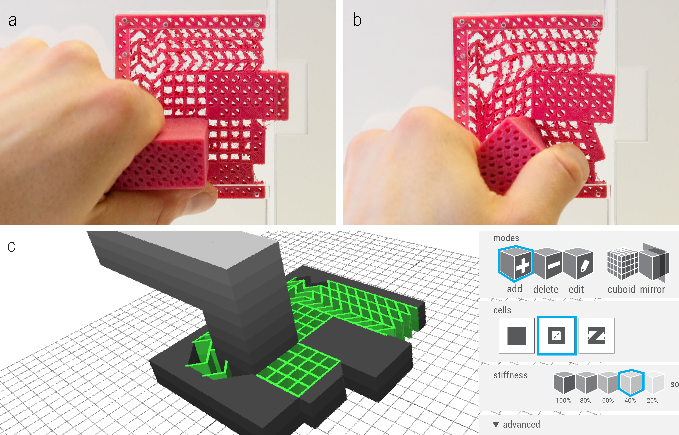
\includegraphics[width=0.85\textwidth]{chapters/introduction-FIG/2-overview-metamaterial-mechanisms.pdf}
    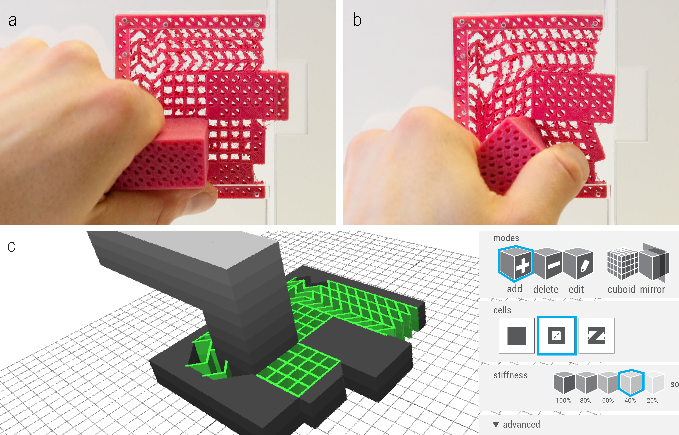
\includegraphics[width=1\textwidth]{chapters/introduction-FIG/2-overview-metamaterial-mechanisms.pdf}
    \caption[Short figure name.]{(a) This door latch demonstrates a metamaterial device that transforms user input, i.e., pushing down the handle, (b) to pulling the latch inwards. (c) We developed a custom editor to assist their design.
    \label{fig:2-overview-metamaterial-mechanisms}}
\end{figure}


The design of metamaterial mechanisms is highly challenging and the extent of mechanisms that can be realized with metamaterials remains unclear. 
We show in Figure \ref{fig:2-1-understanding-constraint-interaction} how a small change can lead to a vastly different output. 
The reason is that a mechanism consists of many cells that are interconnected and impose constraints on each other, the behaviour of the cell structure is unobvious and non-linear. 
To enable novice users to design such metamaterial mechanisms, we implemented a computational design tool takes user-drawn paths as input and optimizes the cell configuration which implements the transformation. 

To achieve this, we dig deeper into the underlying topological constraints of such cell structures and their influence on the resulting mechanism. 
We find that by representing the constraints as a graph we can easily distinguish unique cells configuration. 
For example, Figure \ref{fig:2-1-understanding-constraint-interaction} illustrates that one cell can prevent 7 cells from shearing such that any permutation within these 7 cells creates the same output. 
We bypass these $2^7 = 128$ configurations by only operating on the constraint graph (i.e., merging and splitting connected components), which reduces our search space by several orders of magnitude and ultimately enables such an automatic tool.

% We present an abstraction of the underlying cell structures as a constraint graph, which informs the design of metamaterial mechanisms. For example, we discover that non-linear mechanical transformations can be realized. Based on these findings, we contribute a computational design tool that automatically creates a metamaterial mechanism from user-defined input and output motion paths. This tool is only feasible, because our constraint graph representation highly reduces the search space of possible arrangements of cells. 

\begin{figure} [h] %[h!|H]
    \centering
    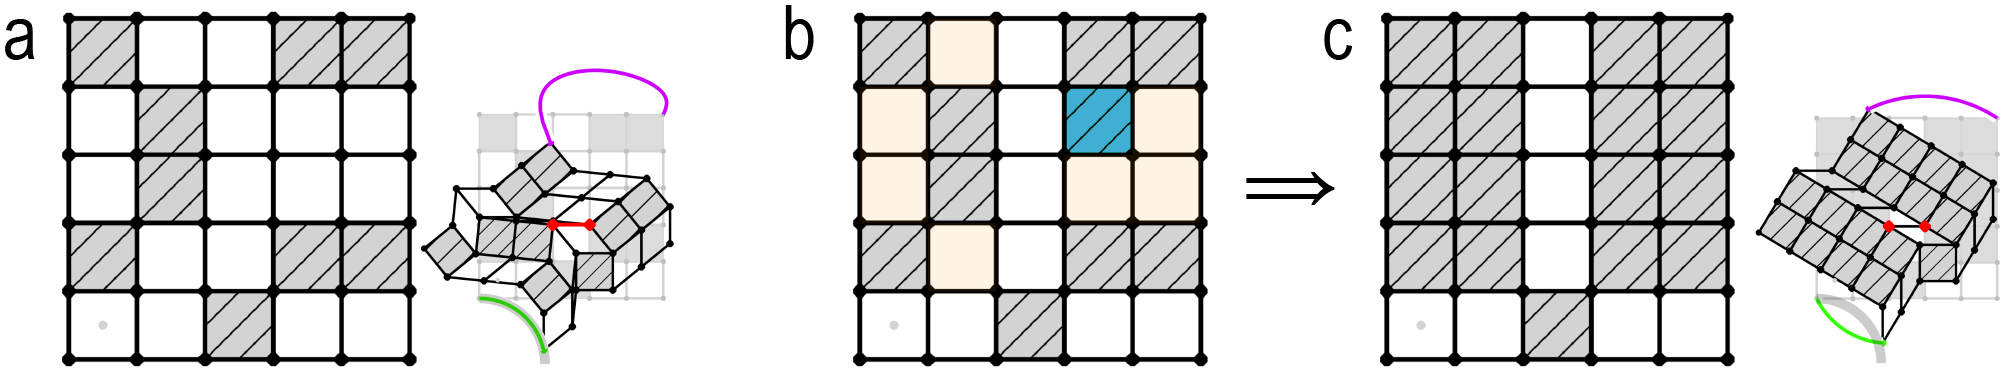
\includegraphics[width=1\textwidth]{chapters/introduction-FIG/2-1-understanding-constraint-interaction.png}
    % 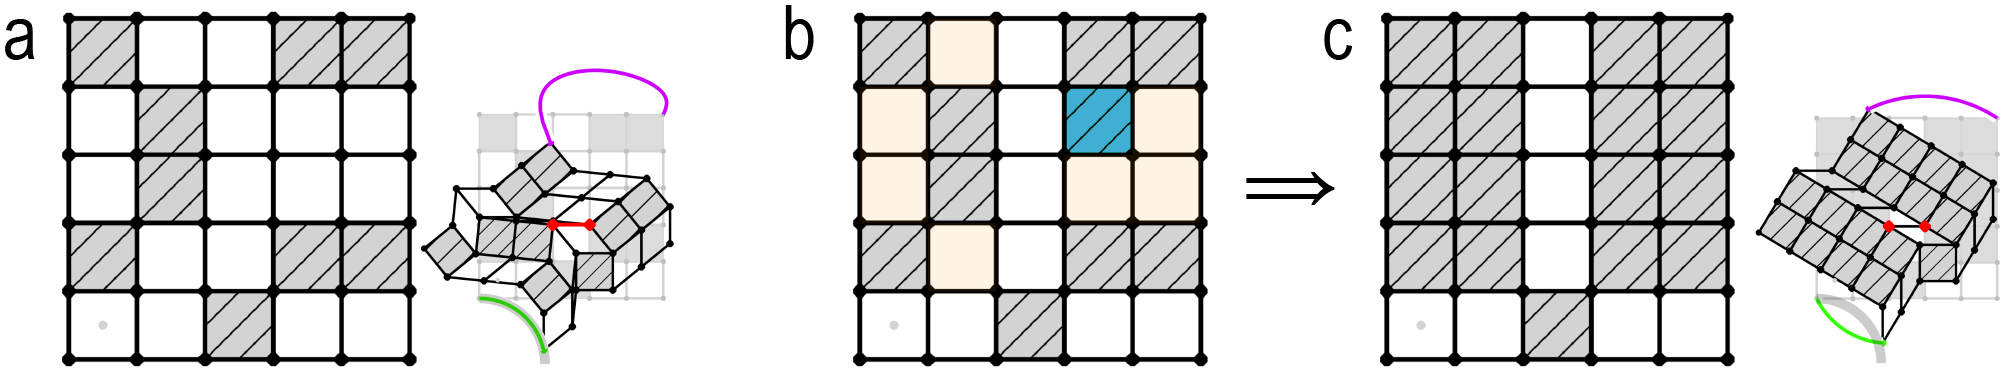
\includegraphics[width=0.85\textwidth]{chapters/introduction-FIG/2-1-understanding-constraint-interaction.png}
    \caption[Short figure name.]{(a) In this example, (b) setting one cell rigid (c) prevents 7 cells from shearing, which changes the output drastically. (c) The green input path from (a) cannot be followed anymore.
    \label{fig:2-1-understanding-constraint-interaction}}
\end{figure}


\subsection{Processing digital signals}

Such analog machines, however, are limited in terms of complexity. As forces are passed on from one cell to the next, they are damped and the activation energy dissipates, causing the mechanical ``signal" to decay. This limits the number of mechanisms that can be concatenated and therefore the complexity of the machine. While this decay can be minimized, it can never be eliminated. This motivated the question `Can we create metamaterials that process digital input, which have no signal decay?' 

To explore this concept, we introduce a new type of cell that propagates a digital mechanical signal, i.e., it counteracts signal decay and thus allows signals to pass through an arbitrary number of cells. Our cell embeds a bistable spring, which discharges when triggered. The resulting impulse triggers one or more neighboring cells, resulting in signal propagation. We extend this basic cell to allow users to implement combinational circuits within 3D printed metamaterial objects. To illustrate this concept, Figure \ref{fig:3-overview-digital-metamaterials} shows a combination lock implemented using digital metamaterials. We contribute 3D printable cells that process signals and make this concept of digital metamaterials accessible to users by extending our specialized 3D voxel-style editor.

\begin{figure} [h] %[h!|H]
    \centering
    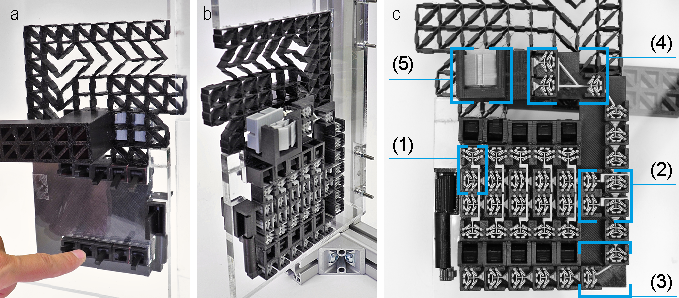
\includegraphics[width=1\textwidth]{chapters/introduction-FIG/3-overview-digital-metamaterials.pdf}
    % 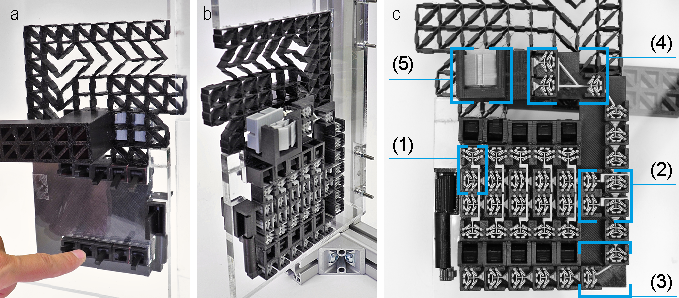
\includegraphics[width=0.85\textwidth]{chapters/introduction-FIG/3-overview-digital-metamaterials.pdf}
    \caption[Short figure name.]{(a) This combination door lock consists of cells that process the code and (b) only unlock the latch if users input the correct code. (c)~Internally, the lock consists of that implement (1) signal validation, (2) logic gates, (3) signal routing, (4) bifurcation, and (5) amplification.
    \label{fig:3-overview-digital-metamaterials}}
\end{figure}


\subsection{Output to the user and the environment}

After investigating two types of metamaterial structures that process information input by the user, we shifted our focus to create metamaterials that \textit{output} to the user. 

We apply the main idea behind metamaterials, i.e., subdivision into a large number of cells and customization on a per-cell basis, to the outsides of 3D printed objects. We introduce metamaterials that undergo a controlled transformation when an external force is applied, allowing users to transition between multiple dynamic textures after fabrication. The resulting metamaterial textures allow designers to shape how the object interacts with the environment and with the tactile sense of the user. Figure \ref{fig:4-overview-textures} shows an example. This door handle transforms its outside, allowing the person behind the door to set three levels tactile messages for everyone trying to enter. The inside of the door handle consists of a grid of cells, which controls how the texture on the object's surface will be formed. 
%We integrated our textured handle with our metamaterial door latch.

\begin{figure} [h]
    \centering
    \includegraphics[width=1\textwidth]{chapters/introduction-FIG/4-overview-textures--2.pdf}
    % 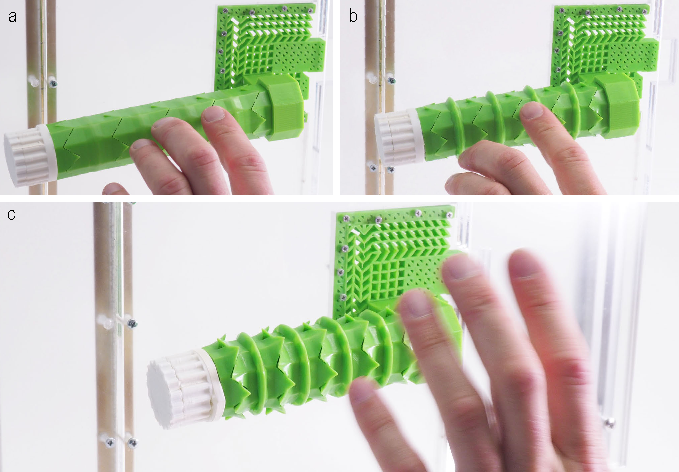
\includegraphics[width=0.85\textwidth]{chapters/introduction-FIG/4-overview-textures.pdf}
    \caption[Short figure name.]{When an external force is applied, metamaterial textures undergo a controlled transformation. This door handle, transforms (a) from flat (b) to rippled (c) to spiky, allowing the person behind the door to set a tactile message with three levels of enter/busy/do not enter messages for visually impaired or sighted users trying to enter.
    \label{fig:4-overview-textures}}
\end{figure}



\section{Contributions}

\textit{The concept of metamaterial devices.} \enspace The main contribution of this thesis is that we apply a radically different thinking to metamaterials. While this emerging field already demonstrated that materials with extreme properties can be engineered by designing their cell structure, we push this further and argue that we can engineer material properties to function as \textit{devices}. 

\textit{Applications and design space.} \enspace We investigated the potential impact and relevance of such metamaterial devices by exploring and building tangible prototypes that can be experiences. These demonstrations inform the potential design space for such devices.

\textit{Cell designs.} \enspace We also contribute a set of cells that enable the realization of metamaterial devices. Our cells include cells that enable a well-defined movement for transmitting forces between cells, they include cells that enable the processing and validation of digital signal and cells that change their outside to interface with the user and the environment.

\textit{Software.} \enspace Lastly, to enable users to create such metamaterial devices, we contribute easily accessible\footnote{open source editor for Metamaterial Mechanisms: \url{https://github.com/jfrohnhofen/metamaterial-mechanisms}} software tools that encapsulate our findings. Our software contains automatic generation of cell assemblies for novice users yet allows experts to freely edit their devices.



\section{Structure of this thesis}

%The structure of this thesis is straight-forward. 
We first give the reader a deeper insight into the current state of the art regarding digital fabrication and metamaterials in Chapter~\ref{chapter:related-work}. Then, in Chapter~\ref{chapter:analog-metamaterials}, we introduce the concept of metamaterial mechanisms. We dive deeper into the structural properties of metamaterial mechanisms in Chapter~\ref{chapter:Understanding-metamaterial-mechanisms}, where we also present a computational design tool that automates the generation of metamaterial mechanisms. We then move on to detailing the structures that enable digital metamaterial devices in Chapter~\ref{chapter:digital}, before explaining how to output to the user by appropriating dynamic textures in Chapter~\ref{chapter:textures}. 
In each chapter, we demonstrate the software that enables users to create such metamaterial devices. 
% In Chapter \ref{chapter:software}, we demonstrate the software that enables users to create such metamaterial devices. 
Lastly, Chapter~\ref{chapter:conclusion} concludes this thesis by discussing the work on a broader level. Since the concept presented in this thesis is novel, it opens up future directions of research, which we  identify and discuss to leave the reader with more food for thought. 
%Lastly, Chapter~\ref{chapter:conclusion} concludes this thesis by discussing the work on a broader level. Since the concept presented in this thesis is novel it opens up future directions of research, which we will identify and discuss in the end of this thesis to leave the reader with more food for thought.



















% something about 3D printers, layer by layer, arrange matter freely in space. 3D printers are solidifiers of digital geometry. Promise the 3rd revolution in manufacturing [economist] and in industrial sense it is getting there [Sculpteo]. but personal fabrication not there, becuase CAD tools are hard to use and hardware is not super reliable. this is why researchers investigate systems.

% % originally, fabrication was mostly concerned iwth the outside; decorative objects but also functional objects of simpler shape (e.g. cast). also due to the fact that 3D printing also comes with their limitations such as speed and support material, thus is also still in development. And designing the shapes also needs some sotware skill. Therefore working on shapes which is the most fail-safe in hardware and software sense, makes sense.  



% % \section{The promise of 3D printing}

% % 3d printing is promising because it can arrange matter freely in space. Does so by a layer by layer approach, thus can make complex geometry without many parts to assemble. other technologies could not, such as laser cutting is 2D and milling needs space for the head to travel.

% % Expected that everyone can make everything. Has printer at home, since they are cheap now. This has not happened yet, mainly because sotfware skill required to design the object and the printers still fail. Researchers work on making 3D printing more accessible and platforms provide models.


% % how great, industrial revolution, slowly happening [Sculpteo]. Personal fabrication less due to 




% % Personal fabrication machines, such as 3D printers, allow users to make custom objects. While early work on 3D printing revolved around designing the outside of such objects [e.g., 35], recently researchers started exploring 3D printing as a means to design the inside of objects. Applications include moving objects’ centers of gravity so as to make them stand [23] or spin [3].

% % Pushing this further, researchers created objects that consist internally of a large number of 3D cells arranged on a regular grid. Since each cell is designed to perform a specific deformation [20], objects that entirely consist of such cells literally offer thousands of degrees of freedom. Such structures are also known as mechanical metamaterials. Metamaterials are artificial structures with mechanical properties that are defined by their usually repetitive cell patterns, rather than the material they are made of [4, 21].

% % Based on this concept, researchers have created objects with unusual behaviors, such as metamaterials that collapse abruptly when compressed [26, 31], that shrink in two dimensions upon one-dimensional compression [28], or objects that mix layers of soft and hard cells in order to emulate different materials [5].


% \subsubsection{From the outside}  
% % \subsubsection{From outside shape}  
% The recent rise of widely accessible fabrication machines, such as 3D printers or laser cutters, generated interest in non-experts to create and design their own devices. Their strive towards a future of personal- rather than mass-fabrication is supported by HCI researchers, who investigate techniques to directly interact with the machine \cite{Mueller2012a}, use real-world objects for content creation \cite{Weichel2014, Weichel2015} or embed mechanisms \cite{Zhang2017} and electronics \cite{Weichel2013, Ledo2017}. These were mainly concerned with creating the outside shape of 3D models.

% \subsubsection{To the inside} 
% % \subsubsection{To static internal structure} 

% % JUST EXPLAIN THESE WORKS IN MORE DETAIL?
% 3D printing technology, however, is unique in that is allows users to freely arrange matter in space. \todo{add netfabb and so} Researchers used this property to generate internal structures that, e.g., optimize the strength to weight ratio of 3D objects \cite{Lu2014}, allow arbitrarily shaped objects to spin reliably \cite{Bacher2014a}, or to float in pre-defined poses \cite{Prevost2016}.

% % \subsubsection{To engineered materials} 
% \subsubsection{To engineered microstructures} 
% Pushing this further, researchers created objects that consist internally of a large number of 3D cells arranged on a regular grid. Since each cell is designed to perform a specific deformation \cite{Overvelde2012a}, objects that entirely consist of such cells literally offer thousands of degrees of freedom. Such structures are also known as mechanical metamaterials. Metamaterials are artificial structures with mechanical properties that are defined by their usually repetitive cell patterns, rather than the material they are made of \cite{Bertoldi2017, Christensen2015, Paulose2015}.

% \todo{add overview of what metamaterials can do, add schumacher}


% % \section{Metamaterial devices: \\defined by their internal structure}
% \section{Metamaterial devices}

% So far, metamaterials have been understood as materials. The main contribution of this thesis is that we want to think of them as \textit{devices.}

% % \todo{add some diagramm that shows this distinction between metamaterials and devices}


% In this dissertation, we push the concept of metamaterials further by creating 3D printed structures inside objects that can process users' input and output to them again, thereby implementing an \textit{input-process-output} system without electronics, but purely within the material structure. The key benefit of our approach is that the resulting objects can be 3D printed from a single material and in one piece and thus do not require assembly.

% % \begin{figure} [h] %[h!|H] 
% %     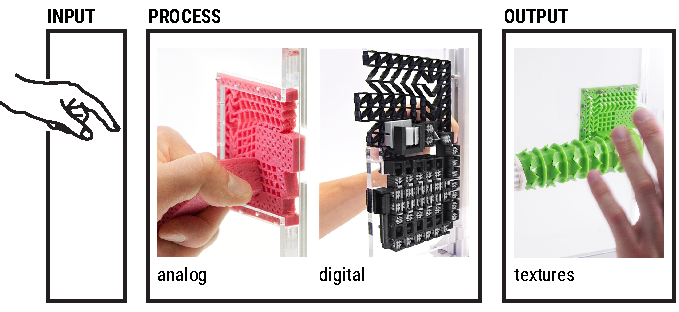
\includegraphics[width=\textwidth]{chapters/introduction-FIG/1-input-process-output.pdf}
% %     \caption[Short figure name.]{Metamaterial devices can process users' input and output to them again, thereby implementing an \textit{input-process-output} system without electronics, but purely within the material structure.
% %     \label{fig:1-overview-input-process-output-model}}
% % \end{figure}

% We contributed cell structures and computational tools that enable users to create 3D printed metamaterial objects capable of processing analog and digital input, as well as to output to the user. 

% \begin{enumerate}
%     \item We integrate mechanisms within the material structure. Such metamaterial mechanisms consist of a single block of material the cells of which play together in a well-defined way in order to achieve macroscopic movement. This allows us to implement, e.g. a door latch, pliers, or a drawing machine from only one piece, without moving parts. 
    
%     \item Going beyond mechanical functions, we explore how to embody mechanical computation into 3D printed objects, i.e., without electronic sensors, actuators, or controllers typically used for this purpose. We demonstrate interactive objects based on this concept, such as a combination lock that are printed in one piece.
    
%     \item To further enhance 3D printed objects, we use metamaterials to change their outside. Such metamaterial textures can perform a controlled transition between two or more textures to allow designers to shape how objects interact with the environment and with the tactile sense of the user. 
% \end{enumerate}

% \todo{and because designing 3D geometry is tricky, as said before, we provide software for these complex metamaterial devices}

% \todo{shorten subsequent sections!}

% \subsection{Processing analog signals}

% In this work, we push the concept of metamaterials further by creating objects that allow for controlled directional movement. This allows users to create objects that perform mechanical functions. Our objects thereby implement devices that transform input forces and movement into a desired set of output forces and movement—also known as mechanisms.

% Figure \ref{fig:2-overview-metamaterial-mechanisms} shows an example of a metamaterial mechanism: a door latch mechanism. Its interior is a regular grid of 3D cells; however, the cells are of different types. Applying a force causes the cells to deform in a controlled way, thereby performing the intended mechanical function. In the example, rotating the door handle causes the cells inside of the object to deform, ultimately pulling the latch towards the left and thereby unlocking the door.

% \begin{figure} [h] %[h!|H]
%     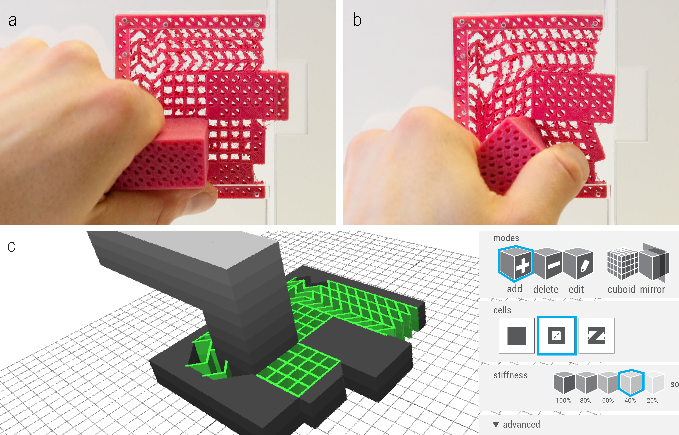
\includegraphics[width=\textwidth]{chapters/introduction-FIG/2-overview-metamaterial-mechanisms.pdf}
%     \caption[Short figure name.]{(a) This door latch is implemented as a metamaterial mechanism; it consists of a single block of material based on a regular grid of cells that together implement handle, latch, and springs. (b) Turning the handle causes the central hinge array to deform and to pull the latch inwards, which unlocks the door. (c) We created this mechanism in our custom editor. Here, we placed two hinge arrays that mechanically couple the handle to the latch, and cells that couple to the doorframe.
%     \label{fig:2-overview-metamaterial-mechanisms}}
% \end{figure}

% While most of the object consists of rigid cells (cells that are reinforced with a diagonal), the object also contains several rectangular regions of cells that lack such a diagonal reinforcement. These are the key to creating mechanisms, as they are able to deform in a very specific way: when subjected to an external force, these cells shear and thereby apply a force to their neighboring cells. 

% Metamaterial mechanisms are simple. While the traditional door latch mechanism consists of several parts, including an axle, bearings, springs, etc., the metamaterial door latch in Figure \ref{fig:2-overview-metamaterial-mechanisms} consists of a single block of material, as it is groups of cells inside the object that perform the mechanical function.

% % While mechanical engineers typically generate metamaterials by scripts [e.g., 21], allowing users of different backgrounds and expertise to create mechanisms requires a dedicated design/engineering process that we argue is best performed by means of an interactive editor. Figure \ref{fig:2-overview-metamaterial-mechanisms}c shows the custom 3D editor we created specifically to allow users to create and modify metamaterial mechanisms. It contains a range of functions that help users assemble specialized cells into basic mechanisms and to assemble such basic mechanisms into more complex mechanisms and simple machines. Using this editor, we have created a series of demo objects including the door latch, a Jansen walker, or a functional pair of pliers. Our examples were printed on a consumer 3D printer (Ultimaker 2+) using a single material.


% \subsection{Processing digital signals}

% Such analog machines, however, are limited in terms of complexity. As forces are passed on from one cell to the next, they are damped and the activation energy dissipates, causing the mechanical ``signal" to decay. This limits the number of mechanisms that can be concatenated and therefore the complexity of the machine. While this decay can be minimized, it can never be eliminated. 

% Therefore, in this work, we explore how to extend this concept towards digital mechanisms, which have no signal decay. Combining metamaterial mechanisms with concepts from mechanical computing and mechanical signal propagation \cite{Raney2016, Nadkarni2014}, we introduce a new type of cell that propagates a digital mechanical signal, i.e., it counteracts signal decay and thus allows signals to pass through an arbitrary number of cells. 
% We introduce a new type of cell that propagates a digital mechanical signal using an embedded bistable spring. When triggered, the embedded spring discharges and the resulting impulse triggers one or more neighboring cells, resulting in signal propagation. We extend this basic cell to allow users to implement combinational circuits within 3D printed metamaterial objects by contributing signal routing, bifurcation, amplification, validation, and logic gates based on 3D printable cells. 

% \begin{figure} [h] %[h!|H]
%     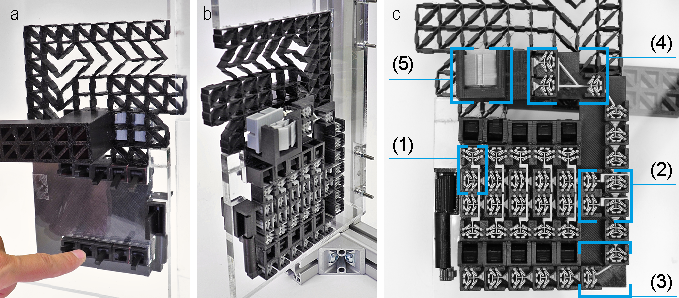
\includegraphics[width=\textwidth]{chapters/introduction-FIG/3-overview-digital-metamaterials.pdf}
%     \caption[Short figure name.]{(a) This combination door lock is implemented as a digital mechanical metamaterial, i.e., a single block of material based on a regular grid of cells. It allows users to input a numeric code, (b) it processes the code, checks its correctness, and unlocks the latch. (c) Internally, the lock consists of an array of cells that transmit and process a mechanical signal.
%     \label{fig:3-overview-digital-metamaterials}}
% \end{figure}

% To illustrate this concept, Figure \ref{fig:3-overview-digital-metamaterials} shows a combination lock implemented using digital metamaterials. The aforementioned shearing cells of the door latch mechanism are blocked by bolts. These bolts are retracted by the digital combination lock only if the user entered the correct 10-digit code. To input the code, users tap one of the 10 digit buttons on the front and push the ‘open’ button, which sets off three signal transmission lines simultaneously; two of which run through the digit evaluation units (Figure \ref{fig:3-overview-digital-metamaterials}c (1)) and set the state of the AND gate (2), which evaluates the correctness of the two rows of digits input by the user. The third signal transmission line is routed (3) from the bottom left towards the right, around the corner, and upwards where the signal is bifurcated (4). This allows triggering a double-sized amplifier cell (5) that actuates the bolts to unblock the door.

% To allow expert users to create and fabricate objects from digital metamaterials, we implemented a specialized 3D voxel-style editor, which is based on the editor for metamaterial mechanisms. The main intent is to allow users to draw signal paths and verify them within the editor. We support users by allowing them to enter simple logic functions, which our editor converts to cell arrangements that implement that function.


% \subsection{Output to the user and the environment}

% In this work, we apply the main idea behind metamaterials, i.e., subdivision into a large number of cells and customization on a per-cell basis, to the outsides of 3D printed objects. The resulting metamaterial textures allow designers to shape how the object interacts with the environment and with the tactile sense of the user.

% We introduce metamaterials that undergo a controlled transformation when an external force is applied, allowing users to transition between multiple dynamic textures after fabrication. Figure \ref{fig:4-overview-textures} shows an example. This door handle transforms from flat to rippled to spiky, allowing the person behind the door to set three levels of enter/busy/do not enter tactile messages for everyone trying to enter. We integrated our textured handle with our metamaterial door latch.

% \begin{figure} [h]
%     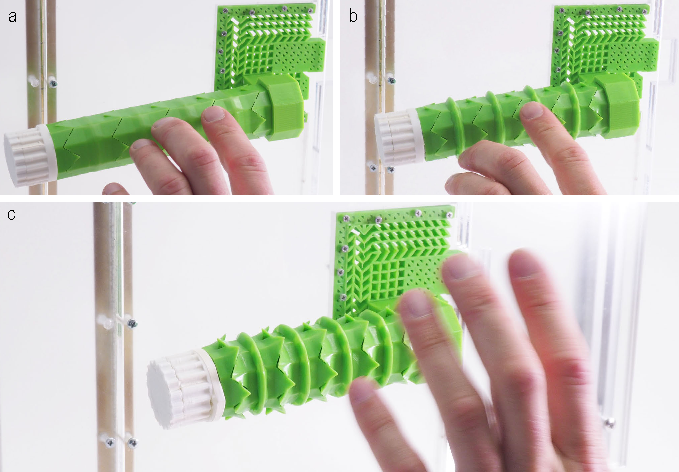
\includegraphics[width=\textwidth]{chapters/introduction-FIG/4-overview-textures.pdf}
%     \caption[Short figure name.]{When an external force is applied, metamaterial textures undergo a controlled transformation. This door handle, for example, transforms (a) from flat (b) to rippled (c) to spiky, allowing the person behind the door to set a tactile message with three levels of enter/busy/do not enter messages for visually impaired or sighted users trying to enter.
%     \label{fig:4-overview-textures}}
% \end{figure}

% The inside of the door handle consists of a grid of cells, which controls how the texture on the object's surface will be formed. We call the underlying cells fold cells. Each cell implements a simple mechanism that transforms horizontal compression into vertical deformation, i.e., it folds upwards when compressed creating a tactile bump. Hence, chaining multiple of these cells allows popping out a texture on the surface of the object. 

% % Beyond this door handle example that uses textures to provides tactile feedback to visually impaired users, such transformable textures allow users to make objects that are adaptable to a specific context such as a shoe sole that transforms from flat to treaded to adapt to weather conditions, or a configurable bicycle grip for exploring parameters during rapid prototyping of textures.

% We present an editor that assists users in creating metamaterial textures interactively by arranging cells, applying forces, and previewing their deformation. Users can achieve a variety of textures by setting the parameters of fold cells, such as hinge offset, width and wall thickness, etc. After having combined their cells, they interactively simulate how the cells deform under continuous compression. Finally, this geometry is exported into a 3D printable .stl file.


% \section{Structure of this thesis}
% \todo{summarize structure}
